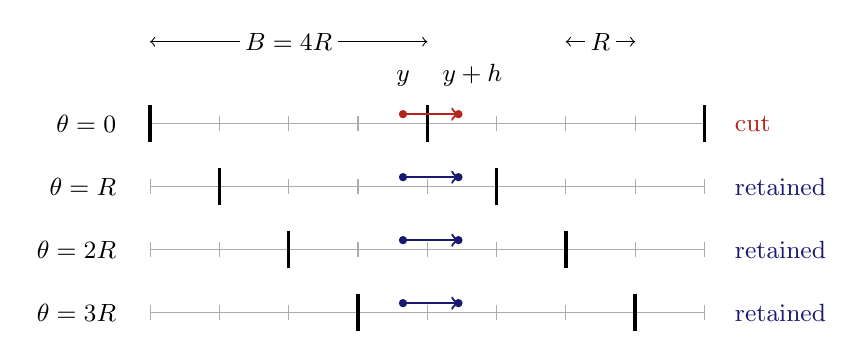
\begin{tikzpicture}[x=.88cm,y=.8cm,font=\small]
 \foreach \row/\shift/\name in {0/0/{0},1/1/{R},2/2/{2R},3/3/{3R}} {
  \begin{scope}[yshift=-\row*0.8cm]
   \node[anchor=east] at (-.35,0) {$\theta=\name$};
   \draw[gray!65] (0,0)--(8,0);
   \foreach \x in {0,...,8} {\draw[gray!65] (\x,-.12)--(\x,.12);}
   \ifnum\row=0
    \foreach \x in {0,4,8} {\draw[very thick] (\x,-.29)--(\x,.29);}
    \draw[->,thick,BrickRed] (3.65,.15)--(4.45,.15);
    \fill[BrickRed] (3.65,.15) circle (1.5pt);
    \fill[BrickRed] (4.45,.15) circle (1.5pt);
    \node[anchor=west,BrickRed] at (8.3,0) {cut};
   \else
    \draw[very thick] (\shift,-.29)--(\shift,.29);
    \draw[very thick] (\shift+4,-.29)--(\shift+4,.29);
    \draw[->,thick,MidnightBlue] (3.65,.15)--(4.45,.15);
    \fill[MidnightBlue] (3.65,.15) circle (1.5pt);
    \fill[MidnightBlue] (4.45,.15) circle (1.5pt);
    \node[anchor=west,MidnightBlue] at (8.3,0) {retained};
   \fi
  \end{scope}
 }
 \node[anchor=south] at (3.65,.43) {$y$};
 \node[anchor=south] at (4.65,.43) {$y+h$};
 \draw[<->] (0,1.3)--(4,1.3);
 \node[fill=white,inner sep=2pt] at (2,1.3) {$B=4R$};
 \draw[<->] (6,1.3)--(7,1.3);
 \node[fill=white,inner sep=2pt] at (6.5,1.3) {$R$};
\end{tikzpicture}
